\section{Scenarii}

Le scénario de fonctionnement de l'application est décrit ci-dessous, ainsi que quelques
cas de dysfonctionnement. Des schémas seront proposés afin de mieux représenter ces enchaînements.

    \subsection{Scenario nominal}
    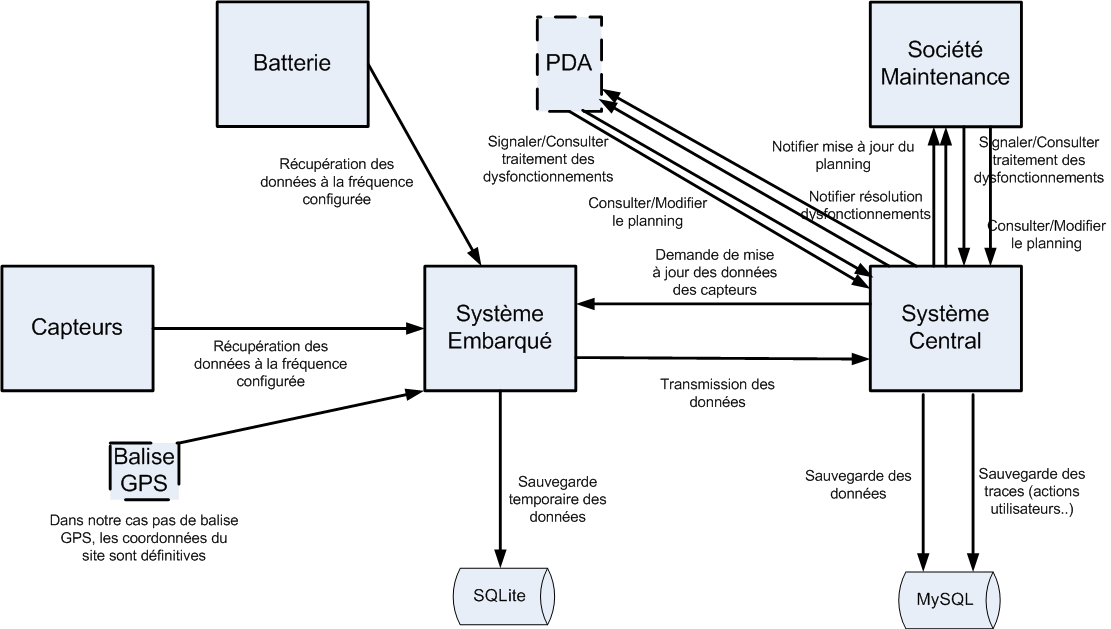
\includegraphics[width = \textwidth] {./img/Cas_Normal.png}
Ce schéma essaye de mettre en évidence l'ensemble des interactions ayant lieu dans un fonctionnement normal.

    \subsection{Scenarii Exceptionnels}

            \subsubsection{Alerte au système central}
            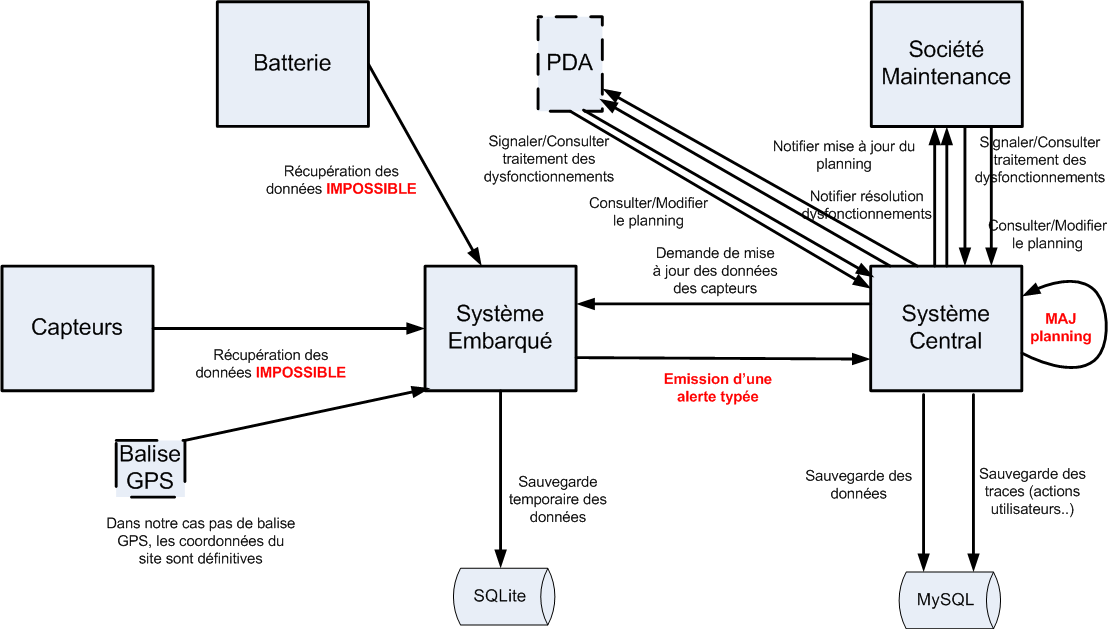
\includegraphics[width = \textwidth] {./img/Alertes.png}
Ce schéma met en évidence les traitements effectués quand le système embarqué détecte un dysfonctionnement.

            \subsubsection{Communication interrompu entre sites générique et central}
            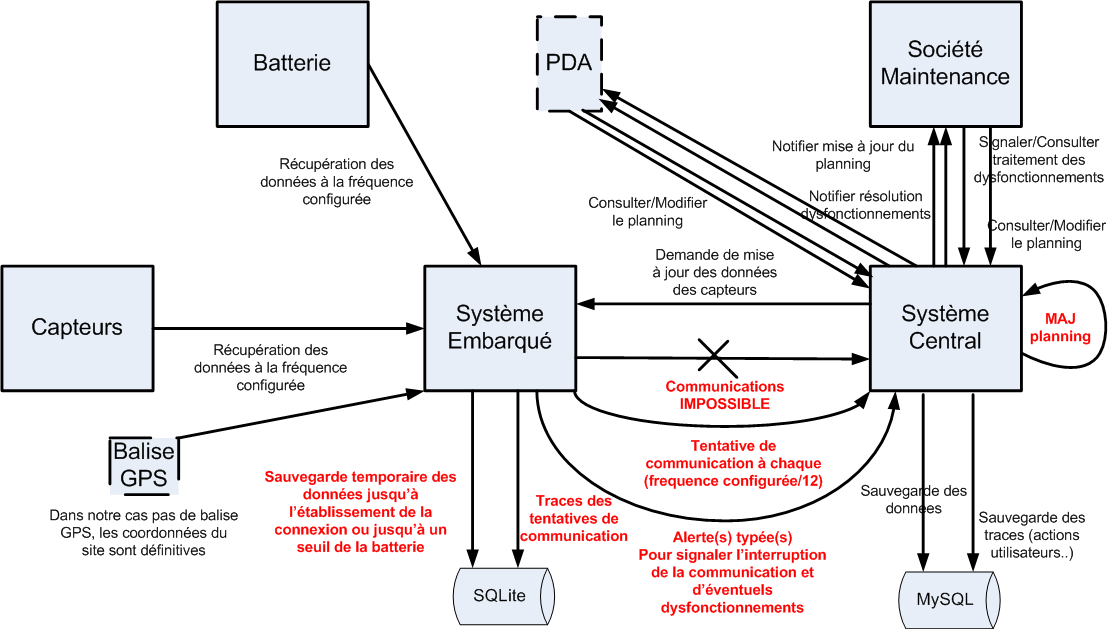
\includegraphics[width = \textwidth] {./img/CommunicationInterrompue.png}
Ce schéma met en évidence les traitements effectués quand le système embarqué n'arrive plus à communiquer 
avec le système central.

On peut imaginer un cas catastrophe ou les communications ne se rétablissement pas et que d'autres problèmes différents de celui de sauvegarde surviennent, par exemple que l'état des batteries soient critiques ou qu'une cuve soit pleine. Dans un souci de zéro défaut, on propose les solutions suivantes sans apporter plus de détails :
 \begin{description}
        \item[État critique de la batterie :] A partir d'un seuil, le système embarqué arrête de récolter les données (des capteurs, de la batterie et de la balise), et s'éteigne afin d'éviter des pertes de données durant son fonctionnement.
        \item[État critique niveau batterie :] On peut imaginer que le système embarqué soit relié à des actionneurs qui permettent d'ouvrir et fermer une vanne; cette vanne pourrait être une vanne d'évacuation pour diminuer le contenu d'une cuve ou ravitailler une cuve.
\end{description}
            \subsubsection{Maintenance à distance}
            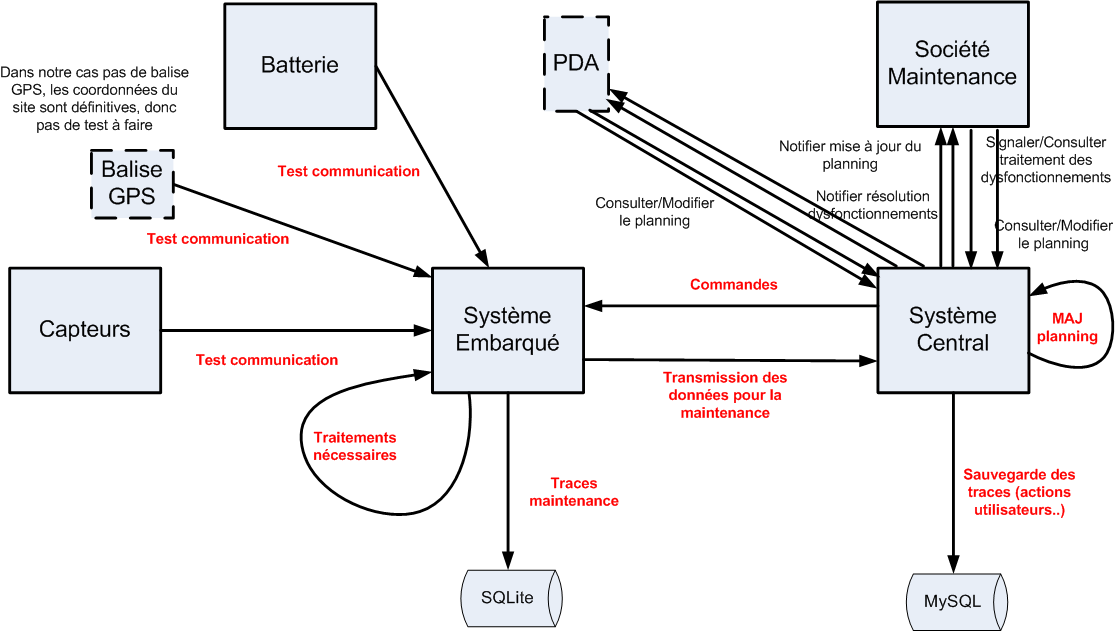
\includegraphics[width = \textwidth] {./img/MaintenanceDistante.png}
Ce schéma met en évidence les traitements effectués quand le système embarqué est maintenu à distance. Les commandes de maintenance seront 
très variées :
\begin{enumerate}
       \item Réinitialiser le système
       \item Vérifier les communications du système avec les capteurs, la source d'énergie, la balise GPS s'il y en a une.
       \item Faire une capture de l'état du système
       \item Tester les protocoles de communication (GPRS, Sattelite, d'autres s'ils en existent..).
 \end{enumerate}
